\documentclass[]{article}
\usepackage{lmodern}
\usepackage{amssymb,amsmath}
\usepackage{ifxetex,ifluatex}
\usepackage{fixltx2e} % provides \textsubscript
\ifnum 0\ifxetex 1\fi\ifluatex 1\fi=0 % if pdftex
  \usepackage[T1]{fontenc}
  \usepackage[utf8]{inputenc}
\else % if luatex or xelatex
  \ifxetex
    \usepackage{mathspec}
  \else
    \usepackage{fontspec}
  \fi
  \defaultfontfeatures{Ligatures=TeX,Scale=MatchLowercase}
\fi
% use upquote if available, for straight quotes in verbatim environments
\IfFileExists{upquote.sty}{\usepackage{upquote}}{}
% use microtype if available
\IfFileExists{microtype.sty}{%
\usepackage{microtype}
\UseMicrotypeSet[protrusion]{basicmath} % disable protrusion for tt fonts
}{}
\usepackage[margin=1in]{geometry}
\usepackage{hyperref}
\hypersetup{unicode=true,
            pdftitle={faoswsStandardization: Full Standardization and Balancing Data-sets content and plug-in execution},
            pdfauthor={Cristina Muschitiello Food and Agriculture Organization of the United Nations},
            pdfborder={0 0 0},
            breaklinks=true}
\urlstyle{same}  % don't use monospace font for urls
\usepackage{graphicx,grffile}
\makeatletter
\def\maxwidth{\ifdim\Gin@nat@width>\linewidth\linewidth\else\Gin@nat@width\fi}
\def\maxheight{\ifdim\Gin@nat@height>\textheight\textheight\else\Gin@nat@height\fi}
\makeatother
% Scale images if necessary, so that they will not overflow the page
% margins by default, and it is still possible to overwrite the defaults
% using explicit options in \includegraphics[width, height, ...]{}
\setkeys{Gin}{width=\maxwidth,height=\maxheight,keepaspectratio}
\IfFileExists{parskip.sty}{%
\usepackage{parskip}
}{% else
\setlength{\parindent}{0pt}
\setlength{\parskip}{6pt plus 2pt minus 1pt}
}
\setlength{\emergencystretch}{3em}  % prevent overfull lines
\providecommand{\tightlist}{%
  \setlength{\itemsep}{0pt}\setlength{\parskip}{0pt}}
\setcounter{secnumdepth}{5}
% Redefines (sub)paragraphs to behave more like sections
\ifx\paragraph\undefined\else
\let\oldparagraph\paragraph
\renewcommand{\paragraph}[1]{\oldparagraph{#1}\mbox{}}
\fi
\ifx\subparagraph\undefined\else
\let\oldsubparagraph\subparagraph
\renewcommand{\subparagraph}[1]{\oldsubparagraph{#1}\mbox{}}
\fi

%%% Use protect on footnotes to avoid problems with footnotes in titles
\let\rmarkdownfootnote\footnote%
\def\footnote{\protect\rmarkdownfootnote}

%%% Change title format to be more compact
\usepackage{titling}

% Create subtitle command for use in maketitle
\newcommand{\subtitle}[1]{
  \posttitle{
    \begin{center}\large#1\end{center}
    }
}

\setlength{\droptitle}{-2em}
  \title{faoswsStandardization:\\
\texttt{Full\ Standardization\ and\ Balancing}\\
Data-sets content and plug-in execution}
  \pretitle{\vspace{\droptitle}\centering\huge}
  \posttitle{\par}
  \author{Cristina Muschitiello\\
Food and Agriculture Organization of the United Nations}
  \preauthor{\centering\large\emph}
  \postauthor{\par}
  \predate{\centering\large\emph}
  \postdate{\par}
  \date{21 June 2018}

\usepackage{lscape}
\usepackage{booktabs}
\usepackage{longtable}
\usepackage{array}
\usepackage{multirow}
\usepackage[table]{xcolor}
\usepackage{wrapfig}
\usepackage{float}
\usepackage{colortbl}
\usepackage{pdflscape}
\usepackage{tabu}
\usepackage{threeparttable}
\usepackage{threeparttablex}
\usepackage[normalem]{ulem}
\usepackage{makecell}

\usepackage{draftwatermark}
\usepackage{makeidx}
\makeindex
\usepackage{float}
\floatplacement{figure}{H}
\usepackage{amsmath}
\usepackage{amssymb}
\usepackage{amsthm}
\usepackage{mathtools}
\usepackage{caption}

\begin{document}
\maketitle
\begin{abstract}
This vignette provides a description on the executin of the ``Full
Standardization and Balancing'' plugin: this is the plugin that,
starting from the data collected and pulled into the input data-set
\texttt{sua\_unbalanced}, performs all the steps of the standardization
and balancing (as described methodologically in a separate document) and
save the data into 3 different output data-sets
\end{abstract}

{
\setcounter{tocdepth}{4}
\tableofcontents
}
\listoffigures

\subsection*{Disclaimer}\label{disclaimer}
\addcontentsline{toc}{subsection}{Disclaimer}

This Working Paper should not be reported as representing the official
view of the FAO. The views expressed in this Working Paper are those of
the author and do not necessarily represent those of the FAO or FAO
policy. Working Papers describe research in progress by the authors and
are published to elicit comments and to further discussion.

This paper is dynamically generated on \today{} and is subject to
changes and updates.

\newpage

\section*{The Data flow}\label{the-data-flow}
\addcontentsline{toc}{section}{The Data flow}

The data Flow of the Standardization and Balancing Plugin is reported in
\ref{fig:f1}. For detail about the methodology, please see the document
\emph{Standardization \& Balancing for Food Balance Sheet Calculation}.

\begin{figure}[H]

{\centering 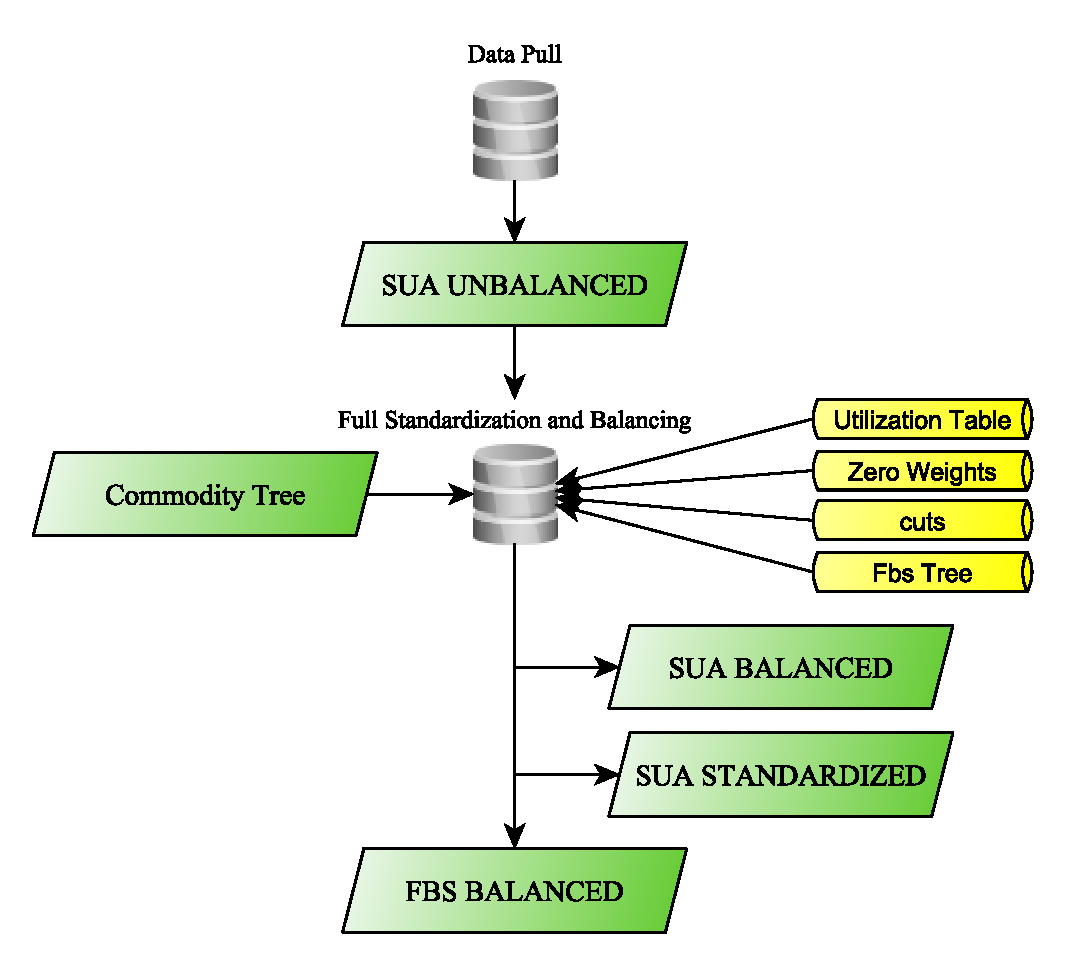
\includegraphics[width=0.7\linewidth]{images/standPlugin/01_dataFlow} 

}

\caption{\label{fig:f1}Data Flow of Standardizatrion and Balancing}\label{fig:f1}
\end{figure}

The \emph{Standardization and Balancing} involves 5 \emph{datasets} and
4 \emph{data tables} in the SWS. One peculiarity of this plug-in is that
is saves data in 3 different data-sets. As a consequence, for executing
it, it is necessary to open 3+1 sessions (3 for the output data-sets and
1 for the input data-set).

\section{Log-in in the SWS}\label{log-in-in-the-sws}

\begin{figure}[H]

{\centering 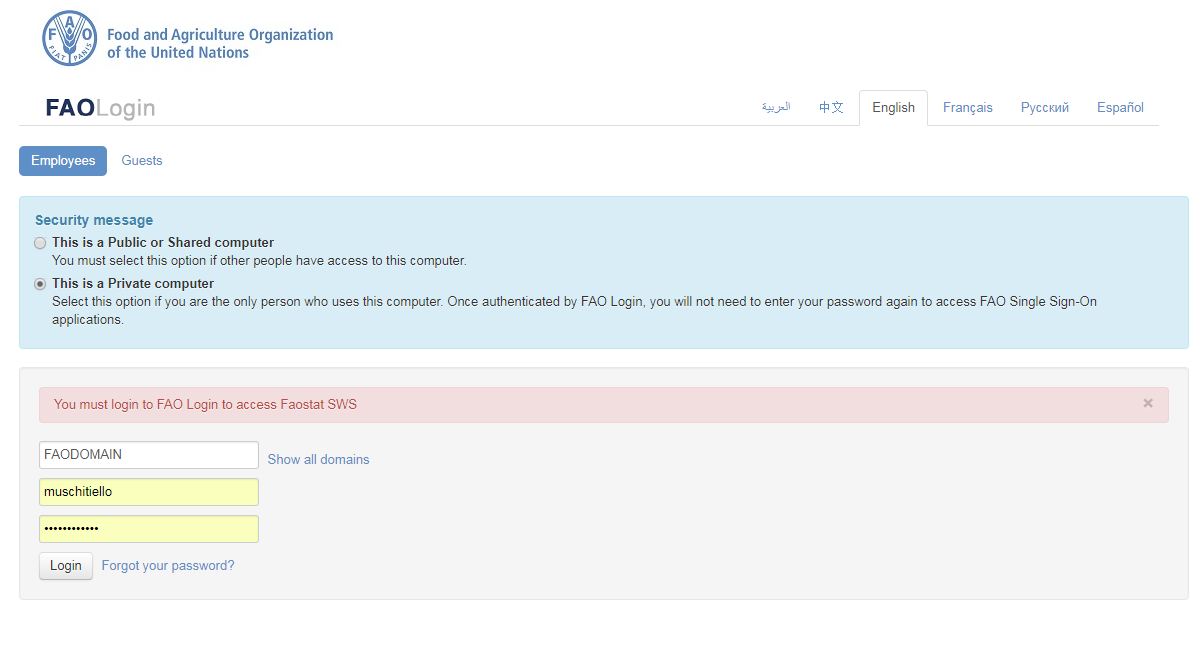
\includegraphics[width=1\linewidth]{images/standPlugin/02_swsLogin} 

}

\caption{\label{fig:f2}Log-in in the SWS}\label{fig:f2}
\end{figure}

\section{Data Pull}\label{data-pull}

First. data from different data-sets have to be pulled inside the
\texttt{sua-unbalanced} data-set and save the data back. This step is
performed trough a plug-in called \texttt{pullDataToSua} which is
documented in a separate document. A general workflow would probably
start from the pulling pf all data for all countries, which are then
saved in the SWS for all the users to start producing FBSs on single
countries.

\section{Open The Sessions.}\label{open-the-sessions.}

4 sessions have to be opened, each one has to be named. This is not
mandatory, but is important enough for reducing confusion and risk error
when the plug-in has to be run. For this document an example on China
Mainland, years from 2010 to 2016 is used.

\subsection{\texorpdfstring{\texttt{sua-unbalanced}
session}{sua-unbalanced session}}\label{sua-unbalanced-session}

This is the session on the \emph{input} data-set. After having used the
\emph{New-session} button, this session has to be opened in the
\emph{suafbs:sua\_unbalanced}. Therefore \emph{SUA/FBS} domain and
\emph{sua\_unbalanced} have to be selected from the screen (figures
\ref{fig:f3} to \ref{fig:f5}).

\begin{figure}[H]

{\centering 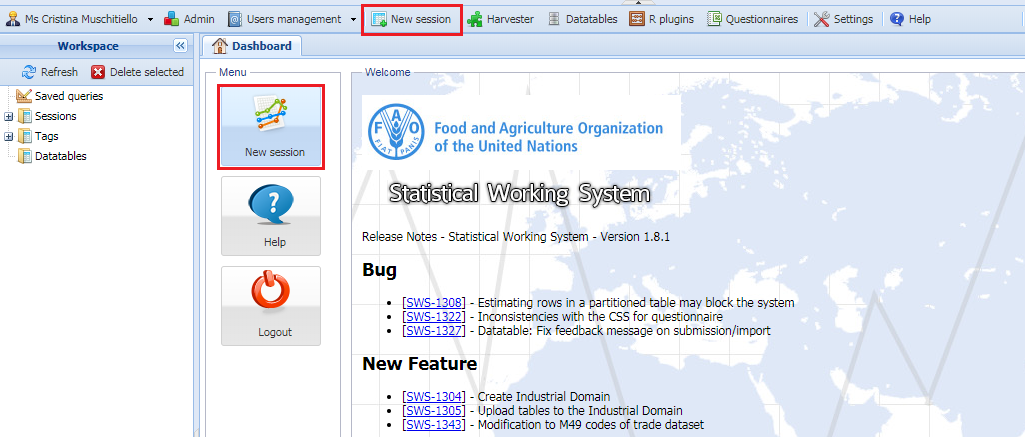
\includegraphics[width=1\linewidth]{images/standPlugin/03_NewSession2} 

}

\caption{\label{fig:f3}Open a new Session}\label{fig:f3}
\end{figure}

\begin{figure}[H]

{\centering 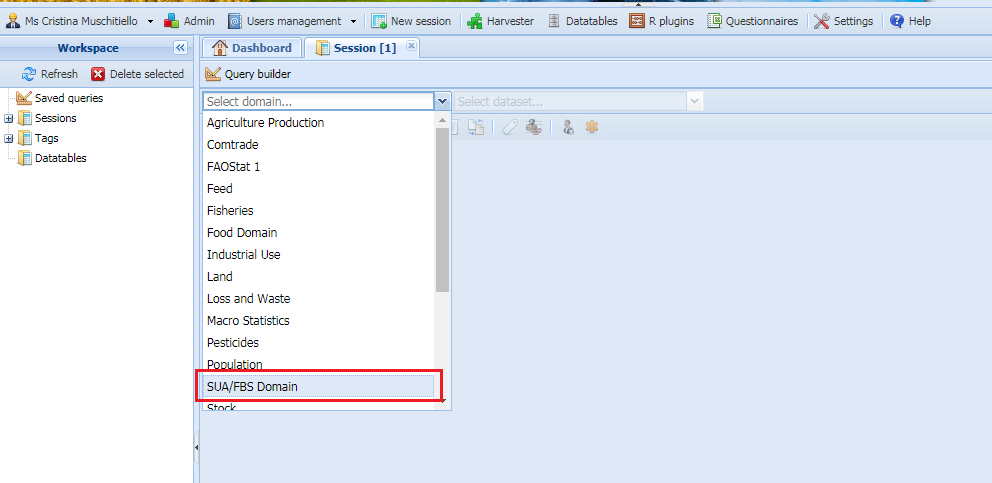
\includegraphics[width=1\linewidth]{images/standPlugin/04_domain} 

}

\caption{\label{fig:f4}Select Domain}\label{fig:f4}
\end{figure}

\begin{figure}[H]

{\centering 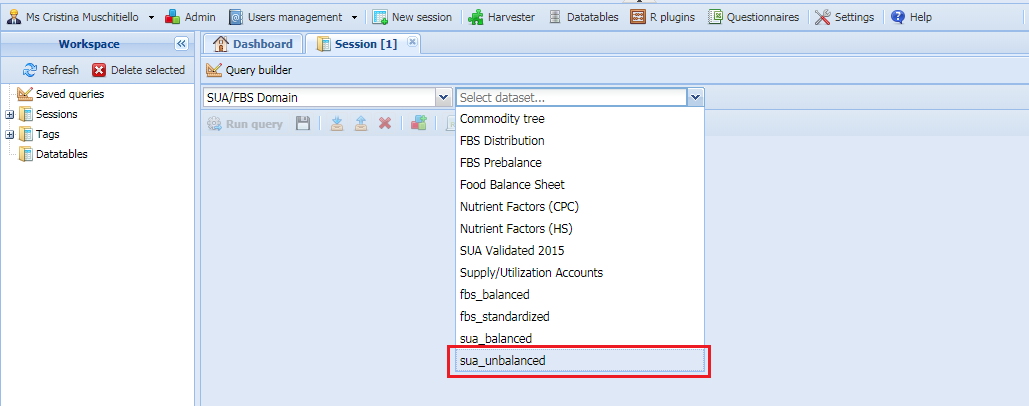
\includegraphics[width=1\linewidth]{images/standPlugin/05_dataset} 

}

\caption{\label{fig:f5}Select Dataset}\label{fig:f5}
\end{figure}

\subsubsection{Make and run the query on this
session}\label{make-and-run-the-query-on-this-session}

The query has to be done only on the country for which the Pull data has
to be performed. Indeed the plugin could be performed on one of the two
following set of countries: \emph{session Countries} or \emph{all
countries}. In our example \emph{China, Mainland} is selected.

\begin{figure}[H]

{\centering 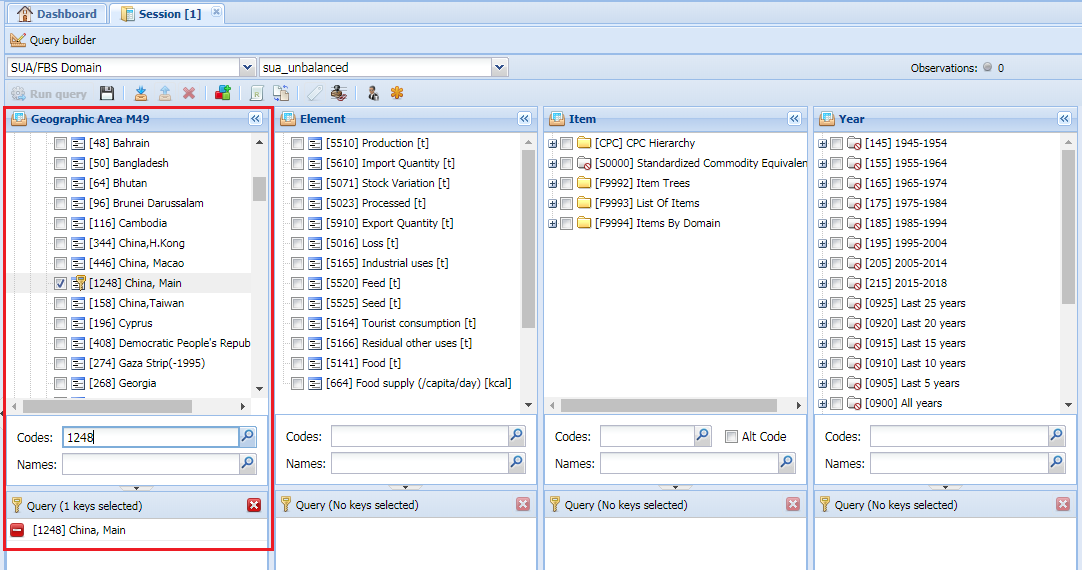
\includegraphics[width=1\linewidth]{images/standPlugin/06_selectCountry} 

}

\caption{\label{fig:f6}Select Country/ies}\label{fig:f6}
\end{figure}

All elements here have to be selected (figure \ref{fig:f7}) and all
items (figure \ref{fig:f8}). The years to be selected depend on the
interest of the user. In this example the time range 2010:2016 is used

\begin{figure}[H]

{\centering 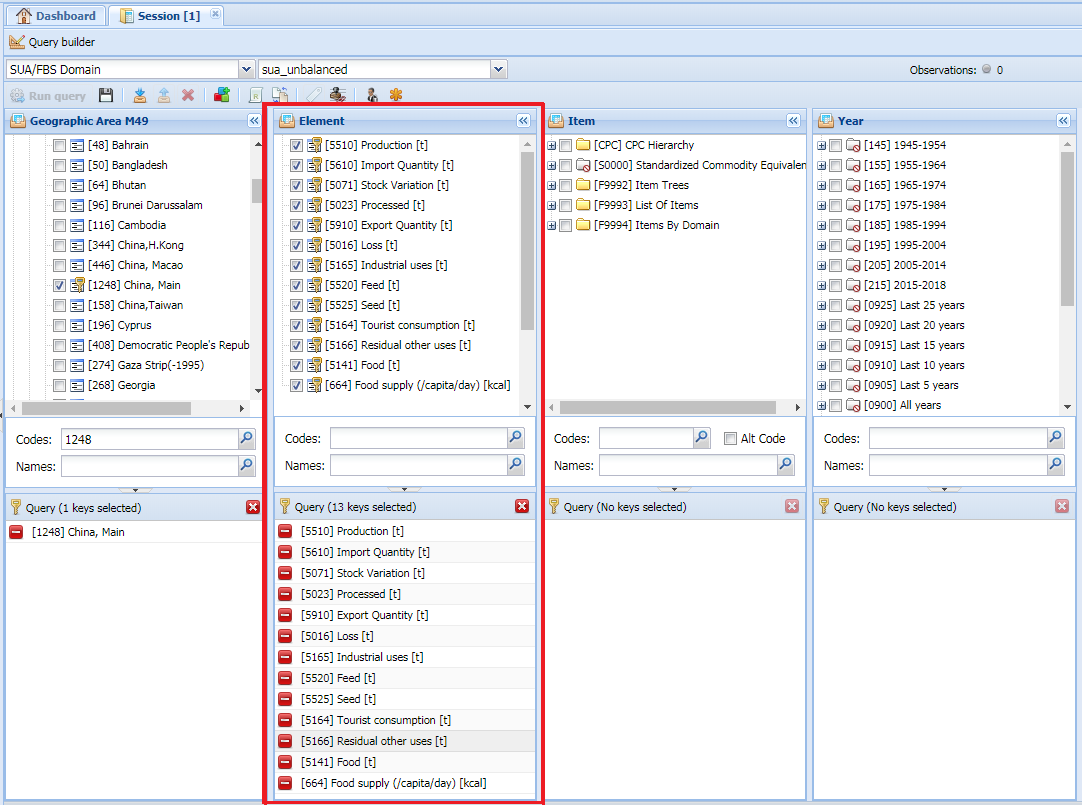
\includegraphics[width=1\linewidth]{images/standPlugin/07_selectElement} 

}

\caption{\label{fig:f7}Select all Elements}\label{fig:f7}
\end{figure}

\begin{figure}[H]

{\centering 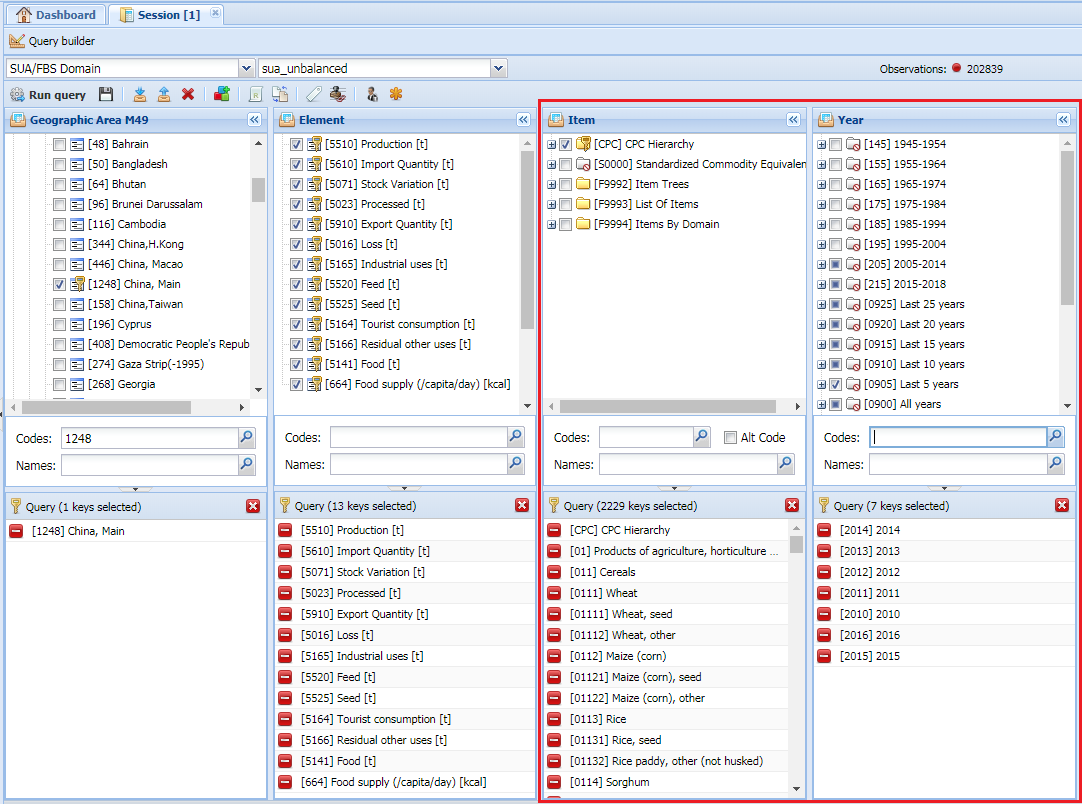
\includegraphics[width=1\linewidth]{images/standPlugin/08_selectItemYear} 

}

\caption{\label{fig:f8}Select items and years}\label{fig:f8}
\end{figure}

When all Variables have been defined, the query can be run:

\begin{figure}[H]

{\centering 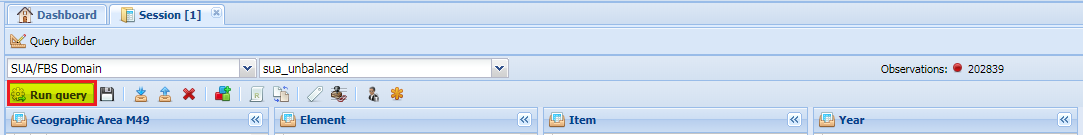
\includegraphics[width=1\linewidth]{images/standPlugin/09_run} 

}

\caption{\label{fig:f9}Run query}\label{fig:f9}
\end{figure}

\subsubsection{The session content}\label{the-session-content}

The Session just created (figure \ref{fig:f10}) contains the data that
will be input of the Plugin for that country. As said in the
\texttt{pullDataToSua} plug-in document\footnote{\emph{faoswsStandardization:\texttt{pullDataToSUA}
  plugin}} ``\emph{At the moment this dataset is filled with data coming
from the old system (dataset ``suaValidated2015''), from 2000 to 2013
for} \textbf{\emph{all countries}} \emph{and New data from 2014
onward}'', if existing. If not existing, because the FBS have not been
calculated yet, there will be blank cells to be filled.

\begin{figure}[H]

{\centering 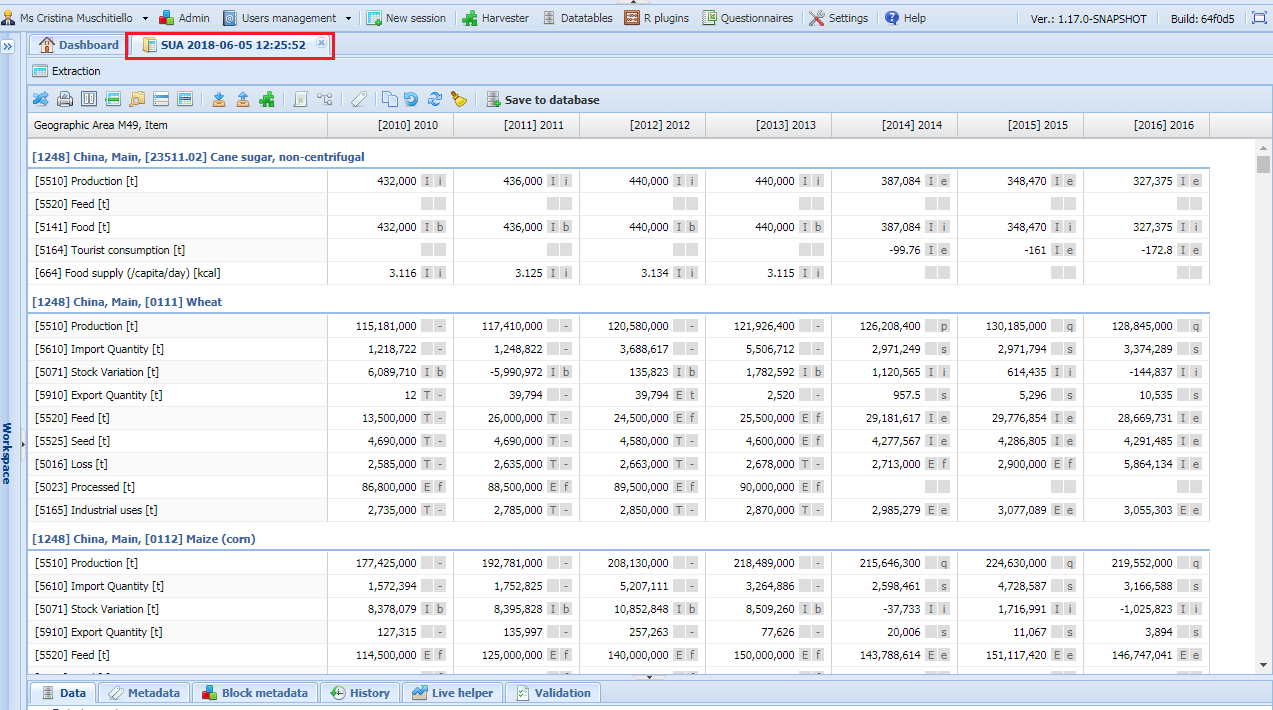
\includegraphics[width=1\linewidth]{images/standPlugin/10_session2} 

}

\caption{\label{fig:f10}The Session}\label{fig:f10}
\end{figure}

As previously mentioned, for the execution of the plugin and an easy
managing of the operations, is better to rename the Session in a
consistent and easily recognizable way.

\subsubsection{Rename session}\label{rename-session}

This session has the name that has been generated automatically from the
SWS: \emph{SUA 2018-06-05 12:25:52} representing the data-set, day and
time of the creation of the Session. As reported in figures
\ref{fig:f11} to \ref{fig:f13}: 1. Right click on the session name 2.
Select ``Rename'' 3. Assign a name 4. click ``ok''

\begin{figure}[H]

{\centering 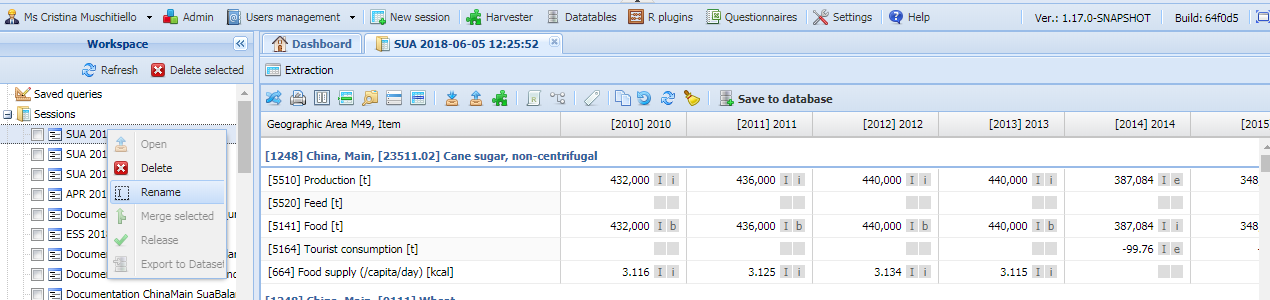
\includegraphics[width=1\linewidth]{images/standPlugin/11_selectRenameSession} 

}

\caption{\label{fig:f11}Rename Session - 1}\label{fig:f11}
\end{figure}

\begin{figure}[H]

{\centering 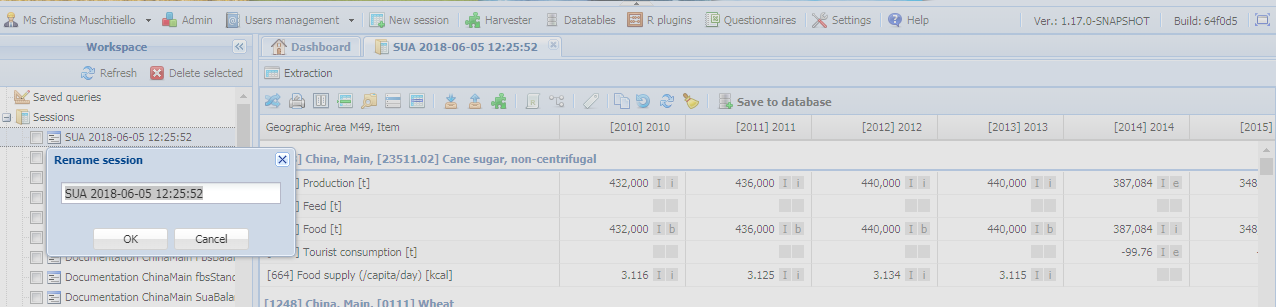
\includegraphics[width=1\linewidth]{images/standPlugin/12_selectDeleteName} 

}

\caption{\label{fig:f12}Rename Session - 2}\label{fig:f12}
\end{figure}

\begin{figure}[H]

{\centering 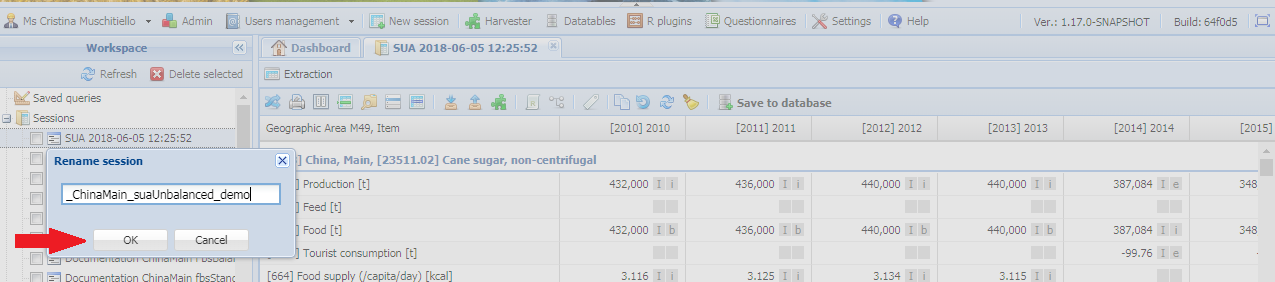
\includegraphics[width=1\linewidth]{images/standPlugin/13_changeName} 

}

\caption{\label{fig:f13}Rename Session - 3}\label{fig:f13}
\end{figure}

\subsection{\texorpdfstring{\texttt{sua-balanced}
session}{sua-balanced session}}\label{sua-balanced-session}

A second session has to be opened on the domain:data-set
\emph{SUA/FBS:sua\_balanced}.

\subsubsection{Make and run the query on the session/Duplicate
Session}\label{make-and-run-the-query-on-the-sessionduplicate-session}

This can be one in two ways. One can re-do all the steps for a new
session, as reported in figures from \ref{fig:f14} to \ref{fig:f17} or
\emph{Duplicate} a session.

\begin{figure}[H]

{\centering 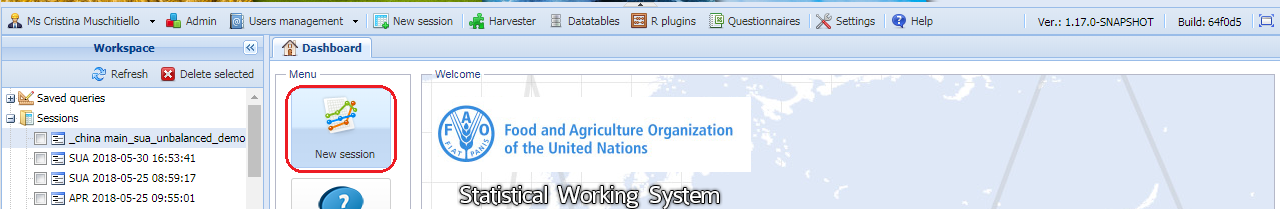
\includegraphics[width=1\linewidth]{images/standPlugin/14_newSession2} 

}

\caption{\label{fig:f14}Sua balanced session - 1}\label{fig:f14}
\end{figure}

\begin{figure}[H]

{\centering 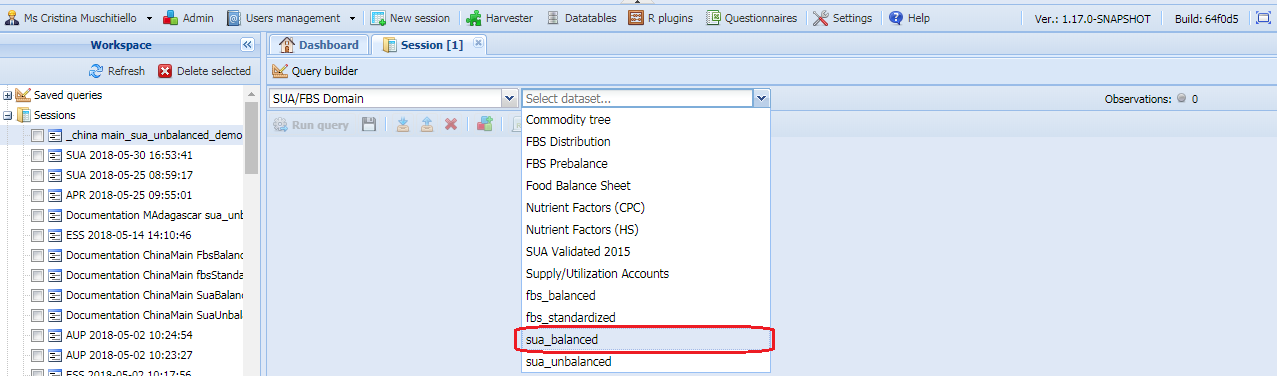
\includegraphics[width=1\linewidth]{images/standPlugin/15_newSession2b} 

}

\caption{\label{fig:f15}Sua balanced session - 2}\label{fig:f15}
\end{figure}

\begin{figure}[H]

{\centering 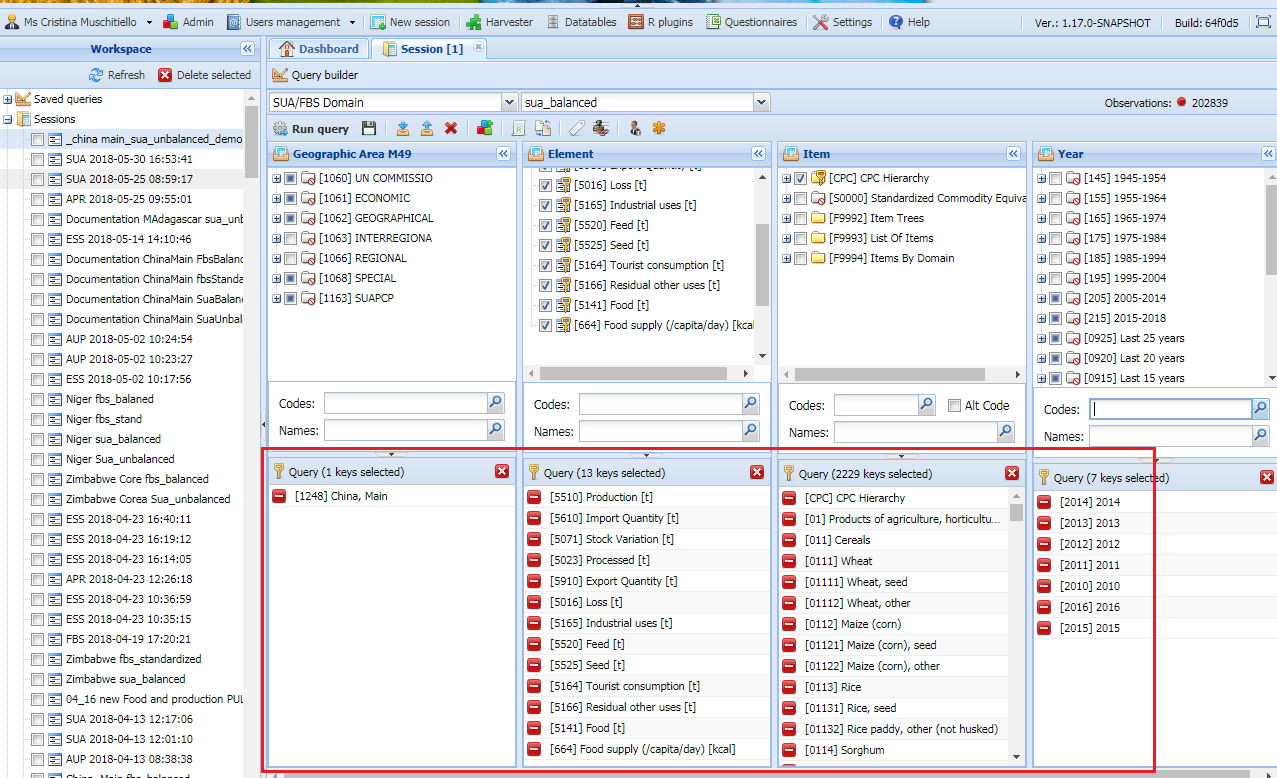
\includegraphics[width=1\linewidth]{images/standPlugin/16_query} 

}

\caption{\label{fig:f16}Sua balanced session - 3}\label{fig:f16}
\end{figure}

\begin{figure}[H]

{\centering 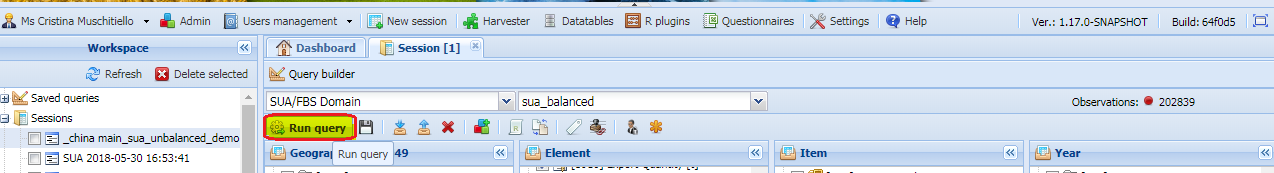
\includegraphics[width=1\linewidth]{images/standPlugin/17_run} 

}

\caption{\label{fig:f17}Sua balanced session - 4}\label{fig:f17}
\end{figure}

Instead of re-doing all these step, an alternative is that of
\textbf{\emph{duplicate}} a session. Indeed, any time one want to create
a session on the same data-set of another or on a different data-set but
same set of data, is possible to select the \emph{duplicate session}
button (figure \ref{fig:f18}). The \emph{Duplicate Session} option open
a new window with a pre-set query identical to the one from which the
session is duplicated. This new pre-set query is still open for changes,
therefore, from here is possible to change the data-set and obtain the
new session without having to select again all the variables. In our
example one should do the \emph{duplicate session} on the
\emph{sua\_unbalanced} table and then change the data-set to
\emph{sua\_balanced} (figure \ref{fig:f19}). This would allow for saving
time in creating the new session on the second data-set, just selection
the desired data-set and then running the query

\begin{figure}[H]

{\centering 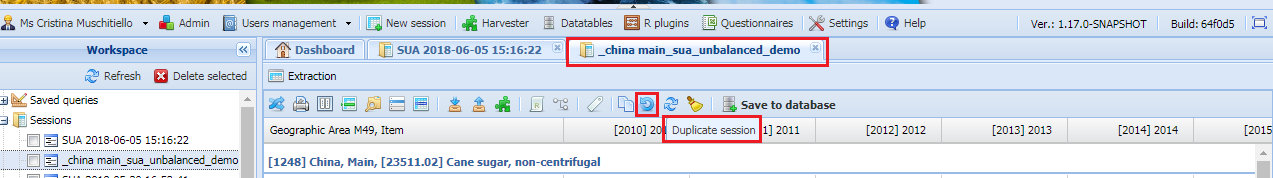
\includegraphics[width=1\linewidth]{images/standPlugin/18_duplicateSession} 

}

\caption{\label{fig:f18}Duplicate Session on sua unbalanced - 1}\label{fig:f18}
\end{figure}

\begin{figure}[H]

{\centering 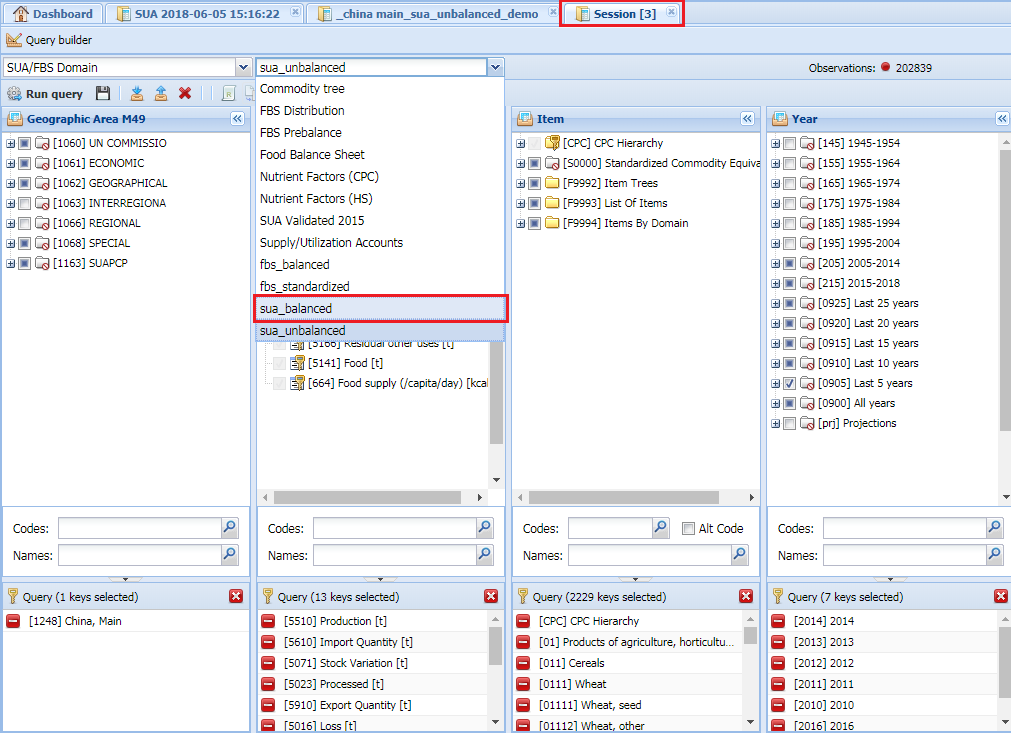
\includegraphics[width=1\linewidth]{images/standPlugin/19_duplicateSession2} 

}

\caption{\label{fig:f19}Duplicate Session on sua unbalanced - 2}\label{fig:f19}
\end{figure}

\subsubsection{Session content}\label{session-content}

Also \emph{sua\_balanced} data-set has been filled with \emph{data
coming from the old system (dataset ``suaValidated2015''), from 2000 to
2013 for} \textbf{\emph{all countries}} \emph{and New data from 2014
onward}.

\subsubsection{Rename session}\label{rename-session-1}

Also this session has to be renamed (figure \ref{fig:f20}).

\begin{figure}[H]

{\centering 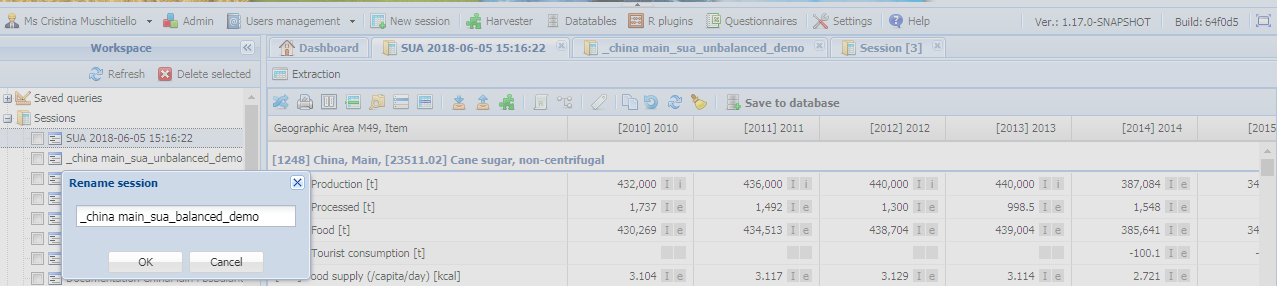
\includegraphics[width=1\linewidth]{images/standPlugin/20_renameBalanced} 

}

\caption{\label{fig:f20}Rename session sua balanced}\label{fig:f20}
\end{figure}

\subsection{\texorpdfstring{\texttt{fbs-standardized}
session}{fbs-standardized session}}\label{fbs-standardized-session}

This session is created using exactly the same steps just explained for
the previous one. After the execution, the session has to be renamed.

\subsubsection{Make and run the query on the session/Duplicate
Session}\label{make-and-run-the-query-on-the-sessionduplicate-session-1}

\begin{figure}[H]

{\centering 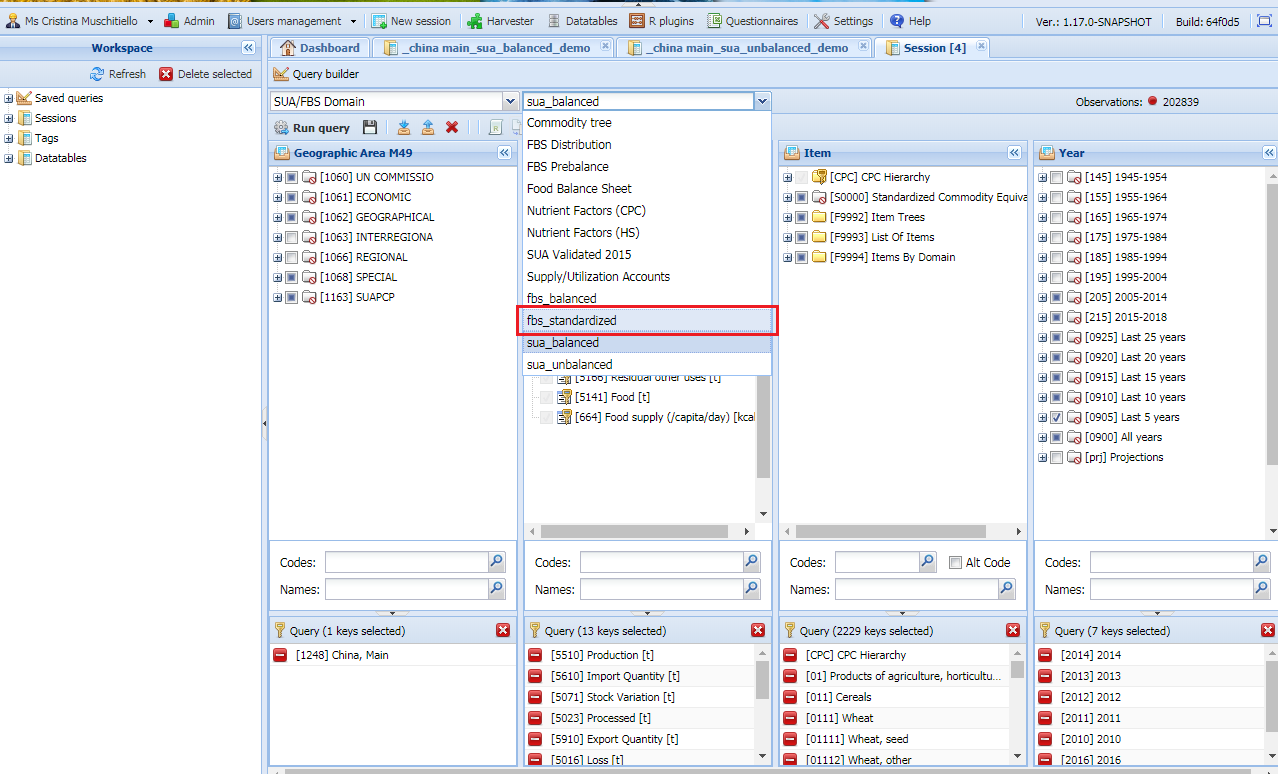
\includegraphics[width=1\linewidth]{images/standPlugin/21_duplicateBalanced} 

}

\caption{\label{fig:f21}Duplicate balanced session in the fbs standardized dataset}\label{fig:f21}
\end{figure}

\subsubsection{Session content}\label{session-content-1}

Because the old system did no have this intermediate step and there was
no old data stored to copy, this data-set has blank valued up to 2013
and new data from 2014. The new data are available for countries that
have been already processed for FBS.

\subsubsection{Rename session}\label{rename-session-2}

\begin{figure}[H]

{\centering 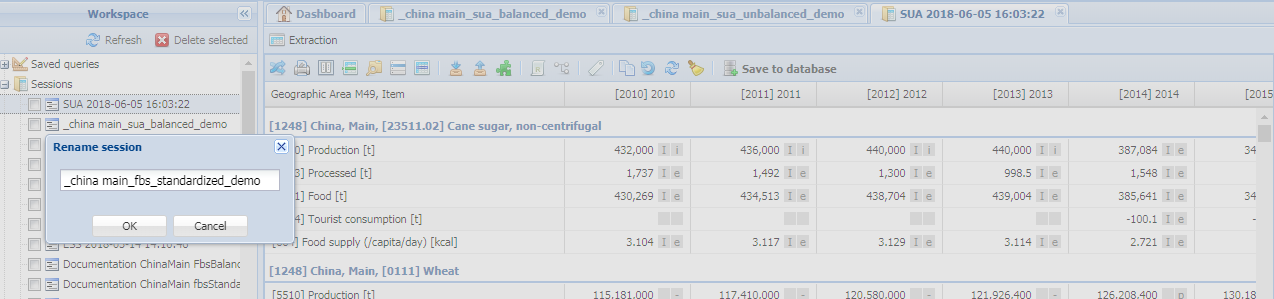
\includegraphics[width=1\linewidth]{images/standPlugin/22_renameStand} 

}

\caption{\label{fig:f22}Rename session fbs standardized}\label{fig:f22}
\end{figure}

\subsection{\texorpdfstring{\texttt{fbs-balanced}
session}{fbs-balanced session}}\label{fbs-balanced-session}

This is the main output data-set.

\subsubsection{Make and run the query on the session/Duplicate
Session}\label{make-and-run-the-query-on-the-sessionduplicate-session-2}

In the use of the \emph{duplicate session} option all the FBS item have
to be selected in addition to the CPC, because this data-set do not
contain CPC item, therefore the session would come empty\footnote{this
  is just a visualization need, in the sense that even if the session is
  empty, it would be filled anyway after the plug-in will be run.
  Anyhow, the previous years would not be visualized if the FBS item are
  not selected}. Also nutritive factors have to be selected in this step
(figure \ref{fig:f23})

\begin{figure}[H]

{\centering 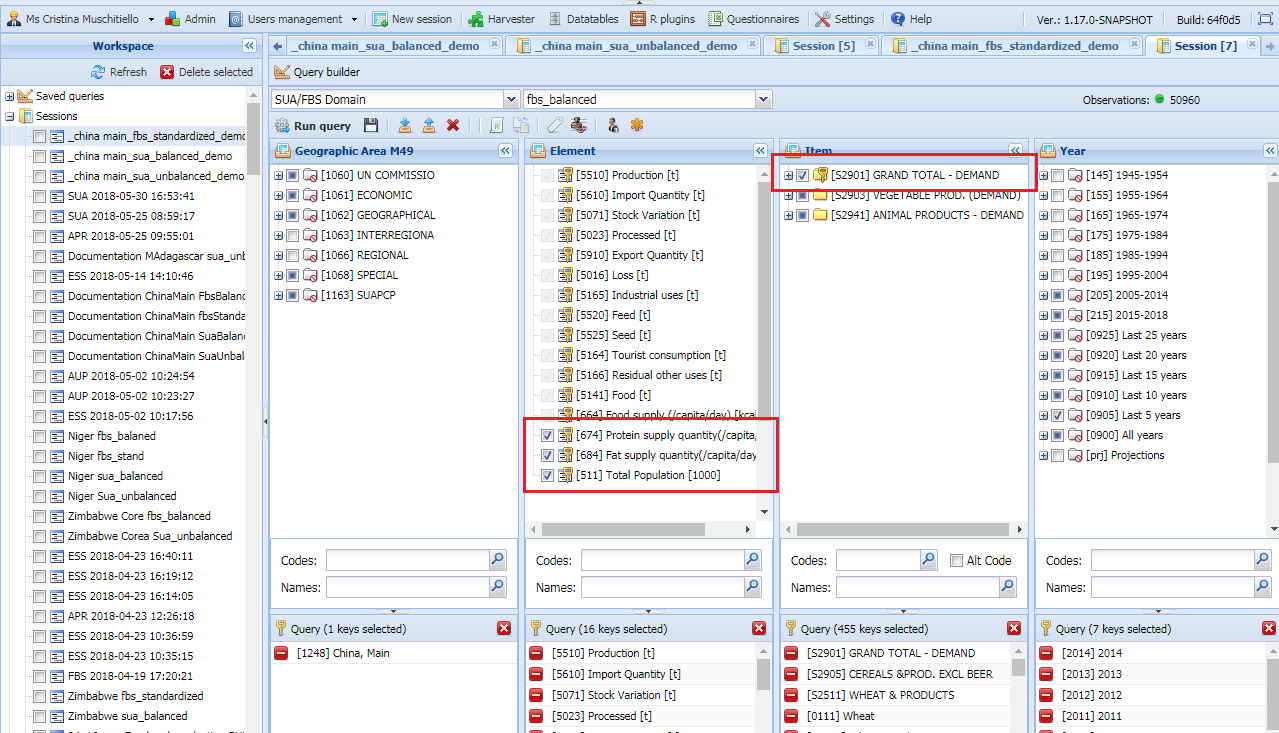
\includegraphics[width=1\linewidth]{images/standPlugin/23_duplicateStandardized} 

}

\caption{\label{fig:f23}Dupicate fbs Standardized}\label{fig:f23}
\end{figure}

\subsubsection{Session content}\label{session-content-2}

FBS data coming from the old System are stored here from 2000 to 2013,
while new FBS data are stored from 2014 onward. The new data are
available for countries that have been already processed for FBS.

\subsubsection{Rename session}\label{rename-session-3}

Rename as the other data-sets.

\begin{figure}[H]

{\centering 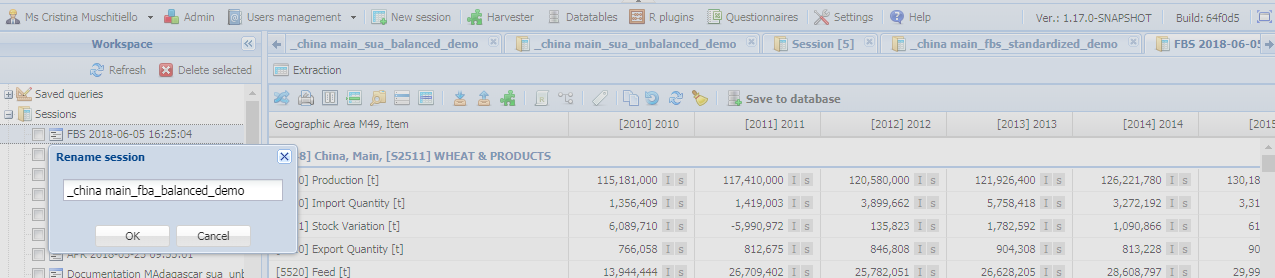
\includegraphics[width=1\linewidth]{images/standPlugin/23_renamefbsBal} 

}

\caption{\label{fig:f24}Rename fbs balanced}\label{fig:f24}
\end{figure}

\section{Select plug-in}\label{select-plug-in}

In the plug-in window, elect the
\texttt{Full\ Standardization\ and\ Balancing} Plug-in. This opens the
window in figure \ref{fig:f27}.

\begin{figure}[H]

{\centering 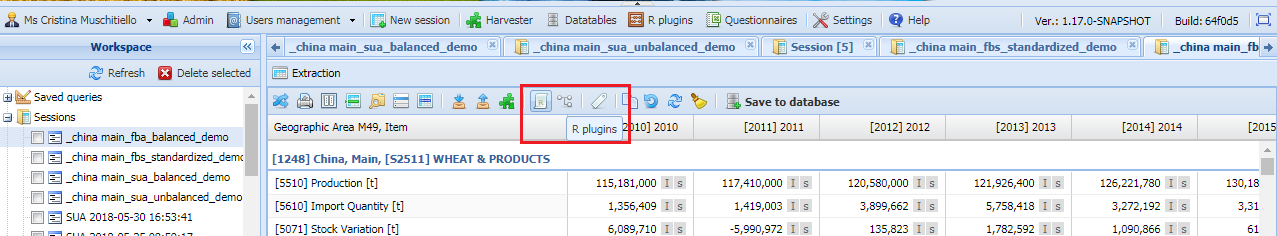
\includegraphics[width=1\linewidth]{images/standPlugin/24_selectPlugin} 

}

\caption{\label{fig:f25}Select plug-in}\label{fig:f25}
\end{figure}

\begin{figure}[H]

{\centering 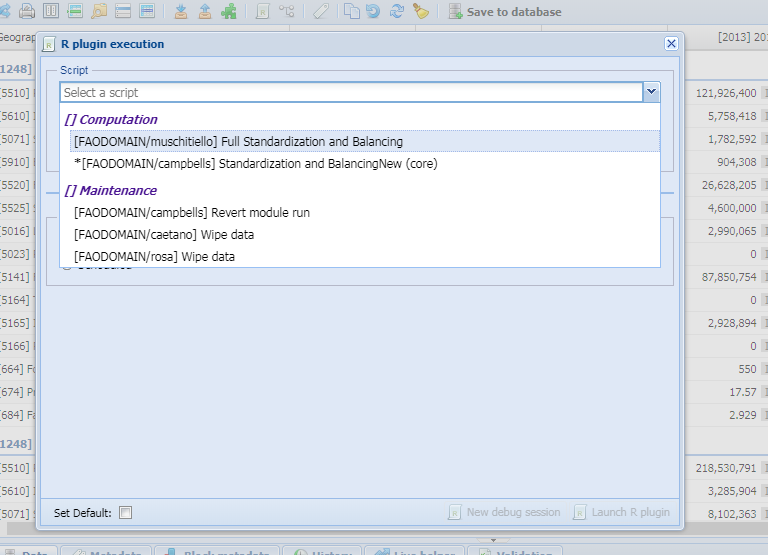
\includegraphics[width=1\linewidth]{images/standPlugin/25_selectPlugin2} 

}

\caption{\label{fig:f26}Plug-in window}\label{fig:f26}
\end{figure}

\begin{figure}[H]

{\centering 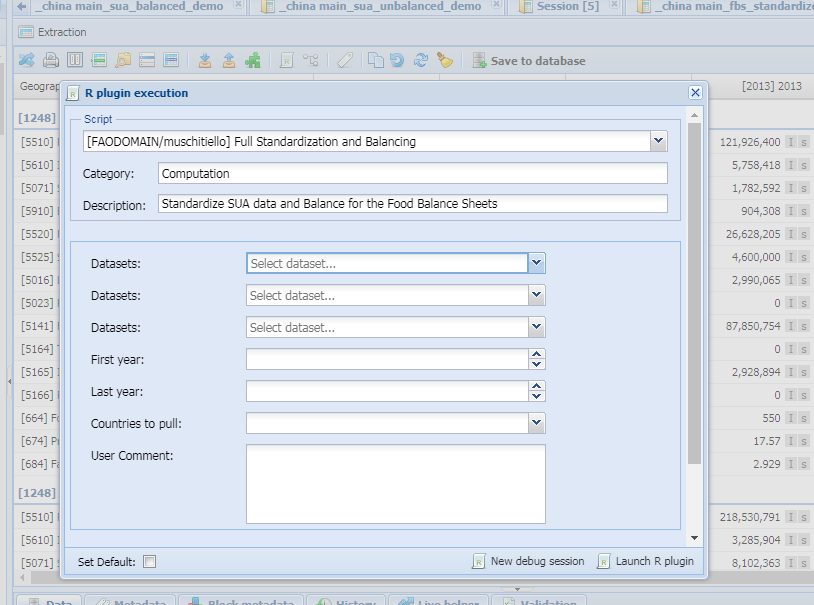
\includegraphics[width=1\linewidth]{images/standPlugin/26_parametersPI1} 

}

\caption{\label{fig:f27}Plug-in parameters - 1}\label{fig:f27}
\end{figure}

There are 3 \emph{Dataset} sections. These are made for specifying the
sessions in which output data have to be saved. The name of the data-set
is reported in the fist line, while the name of the sessions are in the
following lines (figure \ref{fig:f28}). From the drop-down menu, elect
the session you are working in (figures \ref{fig:f28} and
\ref{fig:f29}).

\begin{figure}[H]

{\centering 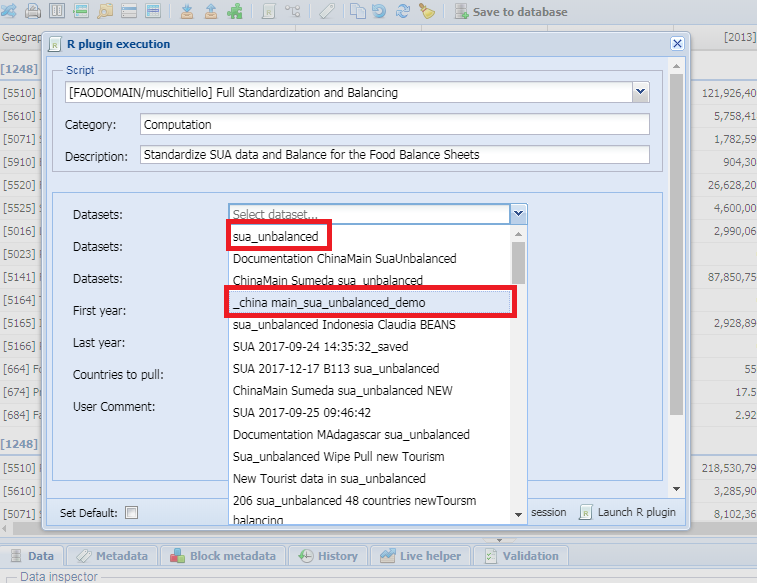
\includegraphics[width=1\linewidth]{images/standPlugin/27_parametersPI2} 

}

\caption{\label{fig:f28}Plug-in parameters - 2}\label{fig:f28}
\end{figure}

Also the time range has to be selected here, which may or may not be the
same as the time range of the session. In this example, the session has
the time range 2010-2016 but the standardization is run for the period
2014-2016.

Finally, also the countries have to be selected. In particular, is
possible to select \emph{all countries} or \emph{session countries}
(figure \ref{fig:f29}).

\begin{figure}[H]

{\centering 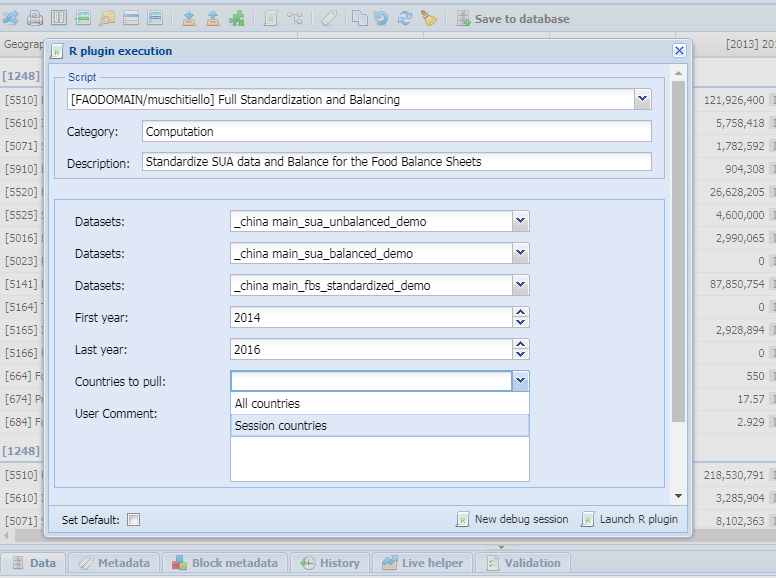
\includegraphics[width=1\linewidth]{images/standPlugin/28_parametersPI3} 

}

\caption{\label{fig:f29}Plug-in parameters - 3}\label{fig:f29}
\end{figure}

After all parameters are set, just launch the plug-in (figure
\ref{fig:f30}).

\begin{figure}[H]

{\centering 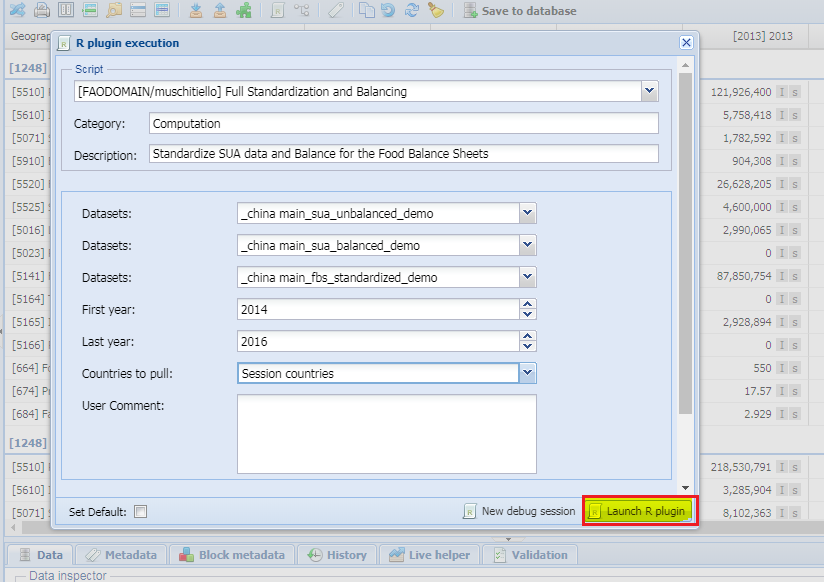
\includegraphics[width=1\linewidth]{images/standPlugin/29_launch} 

}

\caption{\label{fig:f30}Launch Plug-in}\label{fig:f30}
\end{figure}

\section{Plug-in Run}\label{plug-in-run}

While the plug-in runs, some email are sent to the user who launches it:

\begin{enumerate}
\def\labelenumi{\arabic{enumi}.}
\tightlist
\item
  Commodity tree download and check
\end{enumerate}

\begin{quote}
the first email tells that the Commodity tree has been correclty
downoaded. Moreover it also tells that the extraction rates are valid.
This message is sent because the standardization plug-in performs a
validity check on extraction rates. If extraction rates are outside some
specified range or if there are wrong flag combinations, the process
stops. This validation is needed because both \(eR\) and Shares might be
manually changed from any user. If some error is introduced, it has to
be checked otherwise FBS might have inconsistent or wrong results. The
first validation only check extraction Rates. For this reason the
message says taht also a check on shares is needed.
\end{quote}

\begin{figure}[H]

{\centering 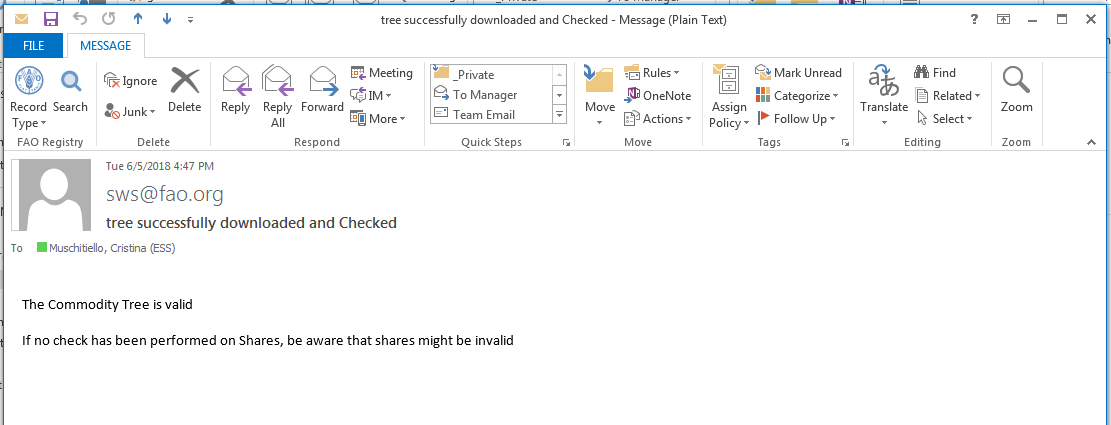
\includegraphics[width=1\linewidth]{images/standPlugin/31_email1} 

}

\caption{\label{fig:f31}Tree Validation email - 1}\label{fig:f31}
\end{figure}

\begin{enumerate}
\def\labelenumi{\arabic{enumi}.}
\setcounter{enumi}{1}
\tightlist
\item
  Check on shares
\end{enumerate}

\begin{quote}
Shares also migh be manually changed by any user. A second check is
introduce for shares. The validation function checks if shares sum up to
1 by child. If the check runs correctly, the email is sent (figure
\ref{fig:f32}), if not, the plug-in stops running. The two checks are
kept separated because the R-functions that perform these validity cheks
might be separatedly needed by other modules and plug-ins\footnote{Developers
  always tries to keep functions general}.
\end{quote}

\begin{figure}[H]

{\centering 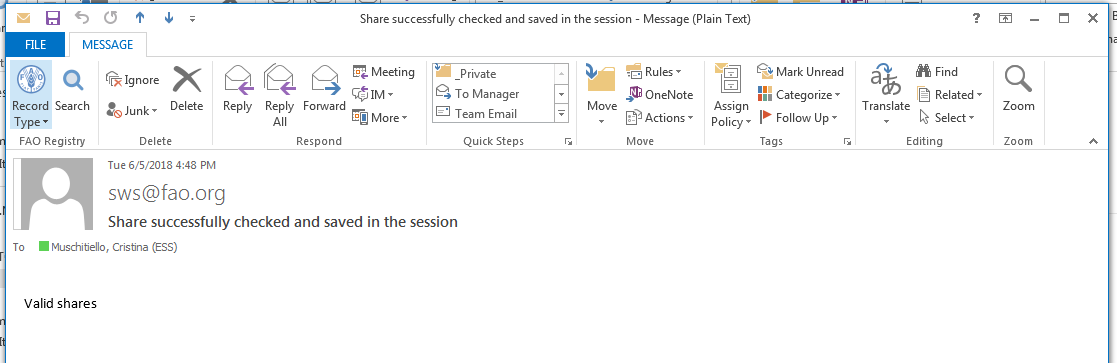
\includegraphics[width=1\linewidth]{images/standPlugin/32_email2} 

}

\caption{\label{fig:f32}Tree Validation email - 2}\label{fig:f32}
\end{figure}

\begin{enumerate}
\def\labelenumi{\arabic{enumi}.}
\setcounter{enumi}{2}
\tightlist
\item
  The plugin runs correctly BUT SOME PRODUCTION FIGURES HAVE BEEN
  CHANGED during the SUA Filling.
\end{enumerate}

\begin{quote}
As discussed, it might happen that, if Utilization \textgreater{}
supplies and it is not enough to reduce utilizations for balancing one
SUA line, the module DO CHANGE OFFICIAL PRODUCTION FIGURES. In this
case, the changed figures are saved in a csv file and sent by email.
This email represents a Warning: Those SUA have to be double-checked and
corrected. An example of the csv file follows. That file contains the
entire SUA in which the production value is changed, by
Country/commodity/year combination. This file is only for visualization.
The changes have to be performed directly in the SWS.
\end{quote}

\begin{enumerate}
\def\labelenumi{\arabic{enumi}.}
\setcounter{enumi}{3}
\tightlist
\item
  Final Email
\end{enumerate}

\begin{quote}
The plug-in may require a lomg time to run, depending on how many
countries are in the session and, also, from the sWS congestion. As a
consequece, the session may expire in the meantime, making it difficult
to understand when the plug-in ends running. The sending of an email
tells when the plug-in has run correctly (\ref{fig:f34}). If the user is
still on the session when it happens, a message is, also visualized on
the screen (\ref{fig:f33}).
\end{quote}

\begin{figure}[H]

{\centering 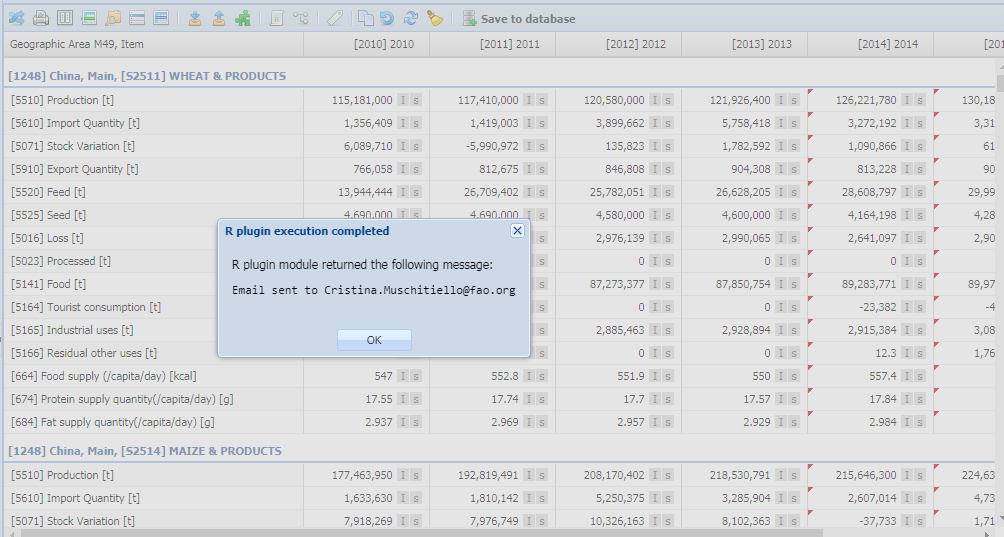
\includegraphics[width=1\linewidth]{images/standPlugin/33_finalEmailmessage} 

}

\caption{\label{fig:f33}Run message}\label{fig:f33}
\end{figure}

\begin{figure}[H]

{\centering 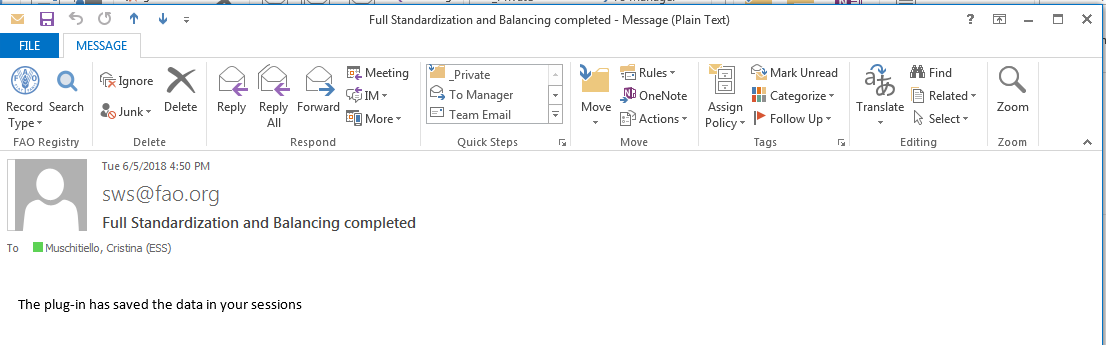
\includegraphics[width=1\linewidth]{images/standPlugin/34_finalEmail} 

}

\caption{\label{fig:f34}Final email}\label{fig:f34}
\end{figure}

\section{The sessions after saving}\label{the-sessions-after-saving}

\subsection{fbs\_balanced session}\label{fbs_balanced-session}

Values have changed IN THE TIME RANGE FOR WHICH THE PLUGIN HAS RUN
(2014:2016), therefore red signs will appear in the cell of the selected
time range. In our example, nothing changes in the time range 2010-2013
(\ref{fig:f35}).

\begin{figure}[H]

{\centering 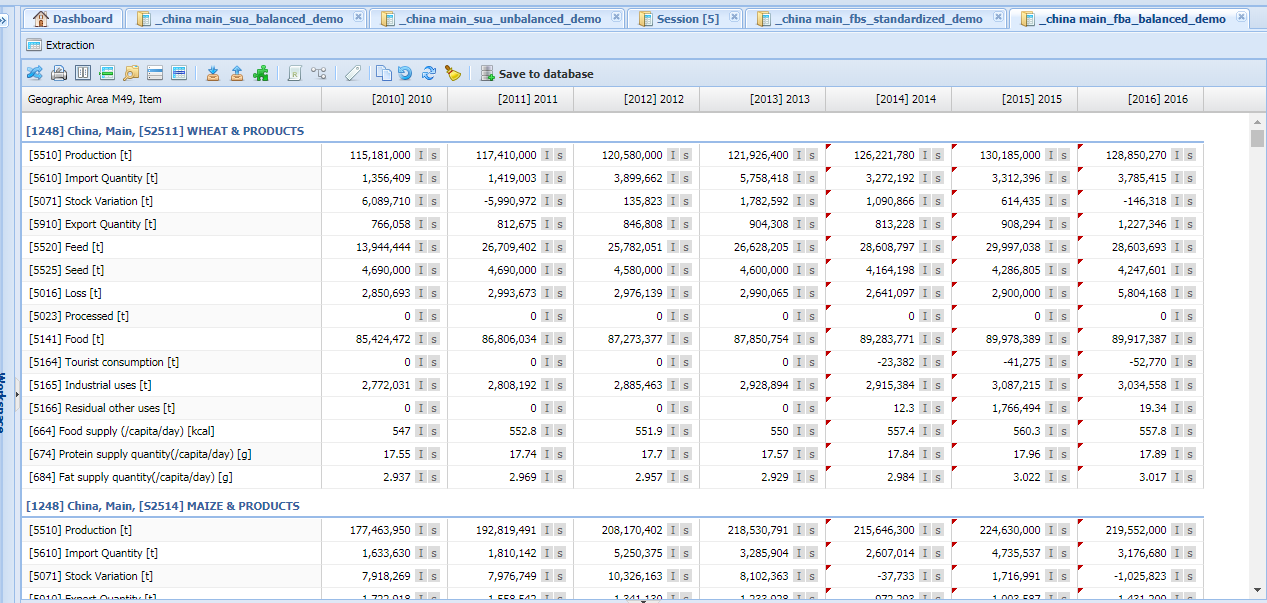
\includegraphics[width=1\linewidth]{images/standPlugin/35_finalSession} 

}

\caption{\label{fig:f35}The session after the Run}\label{fig:f35}
\end{figure}

\subsection{fbs\_standardized session}\label{fbs_standardized-session}

Values have changed IN THE TIME RANGE FOR WHICH THE PLUGIN HAS RUN
(2014:2016), therefore red signs will appear in the cell of the selected
time range. In our example, nothing changes in the time range 2010-2013
(\ref{fig:f36}).

\begin{figure}[H]

{\centering 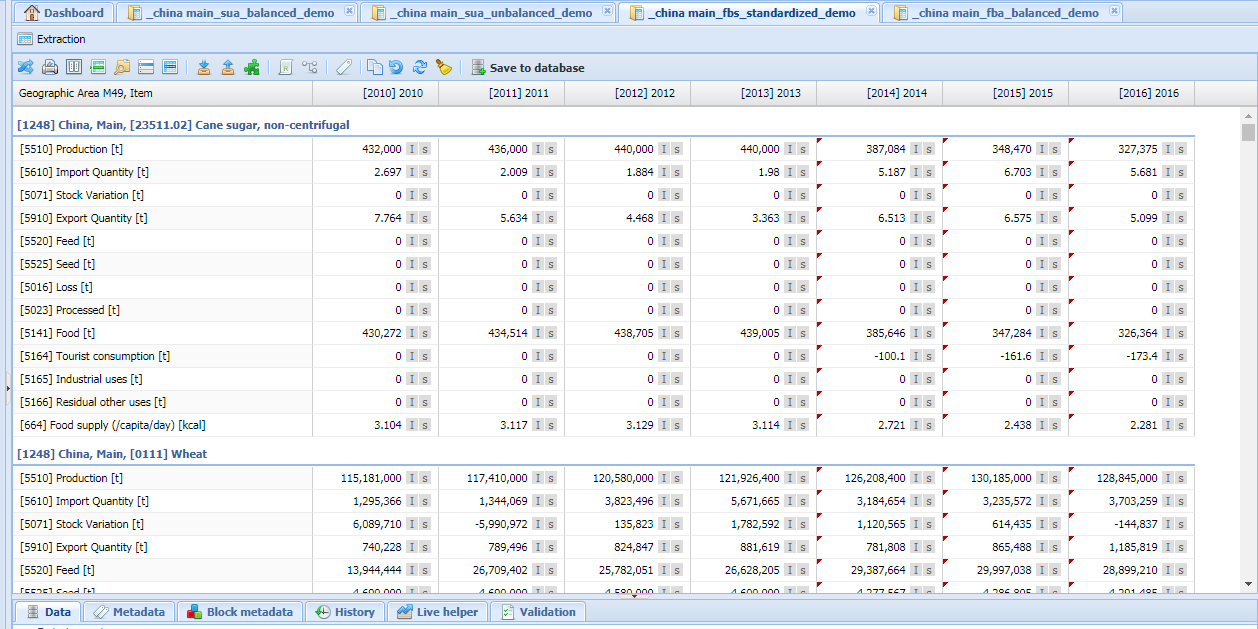
\includegraphics[width=1\linewidth]{images/standPlugin/37_fbsStandAfter} 

}

\caption{\label{fig:f36}fbs standardized after the plug-in run}\label{fig:f36}
\end{figure}

\subsection{sua\_balanced session}\label{sua_balanced-session}

Here values have changed IN THE TIME RANGE FOR WHICH THE PLUGIN HAS RUN
(2014:2016), therefore red signs will appear in the cell of the selected
time range. Nothing is changed in the other time ranges, instead: the
same data as sua\_unbalanced are shown for years up to 2013.

\begin{figure}[H]

{\centering 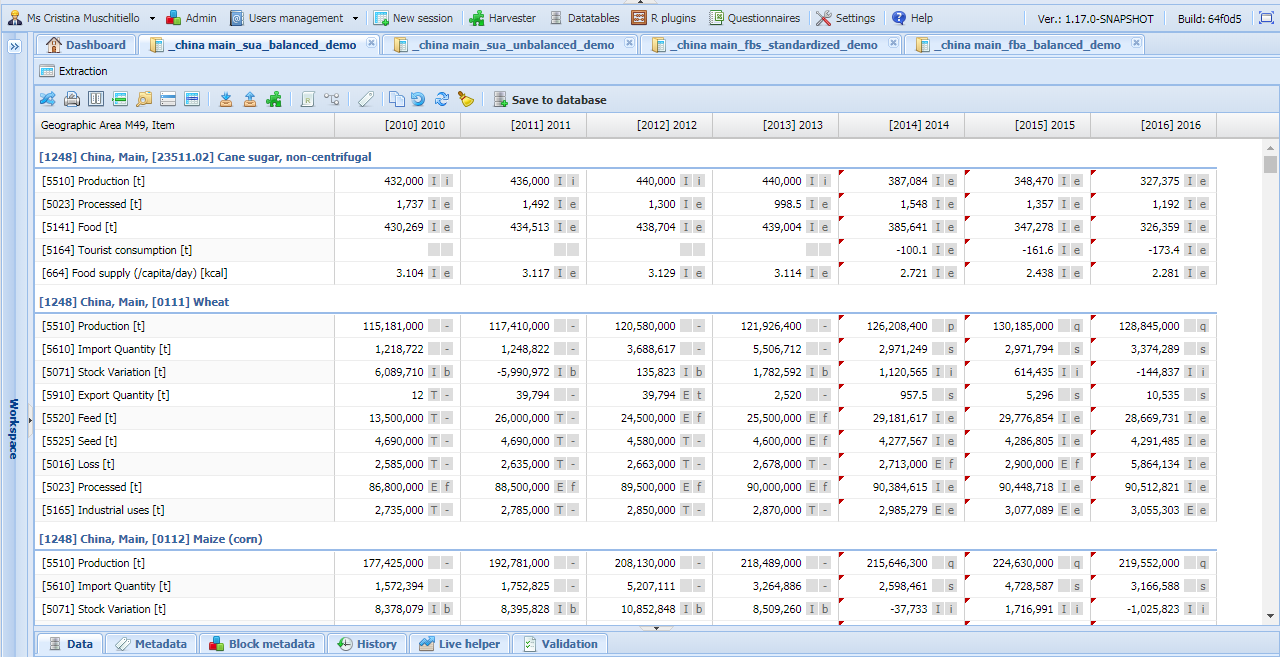
\includegraphics[width=1\linewidth]{images/standPlugin/38_suaBalancedAfter} 

}

\caption{\label{fig:f37}sua balanced after the plug-in run}\label{fig:f37}
\end{figure}

\subsection{sua\_unbalanced session}\label{sua_unbalanced-session}

This is the input data-set, therefore no changes in values happen in
this table.

\section{Final Save into the SWS}\label{final-save-into-the-sws}

For the new figures to be used in following steps, the data have to be
saved to the database.

\begin{figure}[H]

{\centering 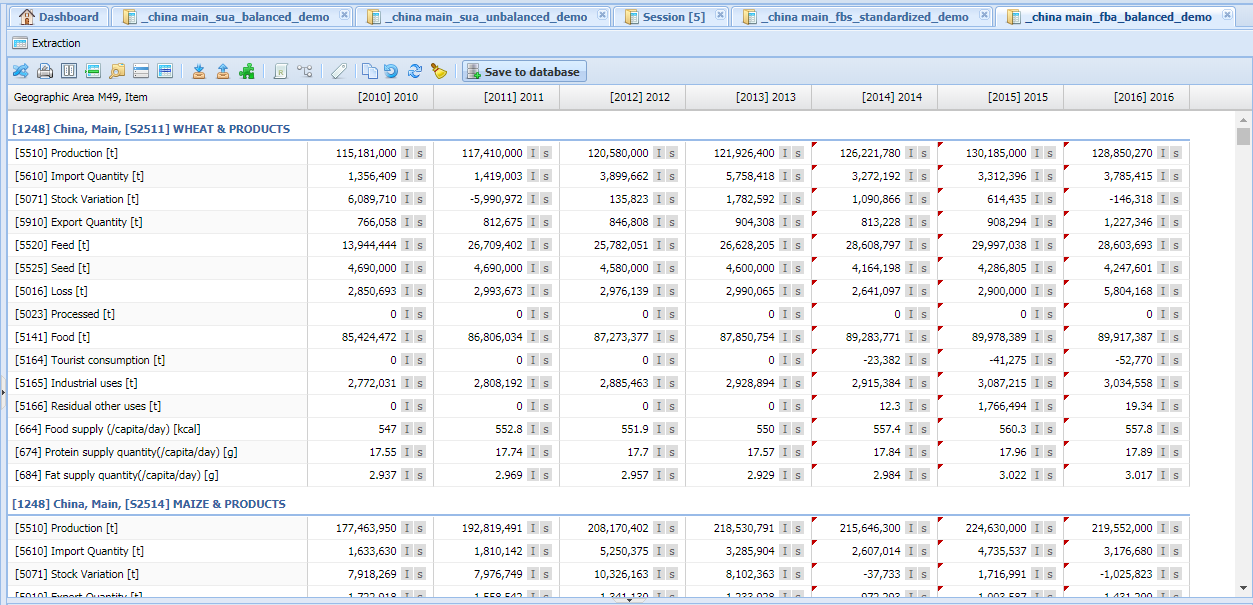
\includegraphics[width=1\linewidth]{images/standPlugin/36_saveBack} 

}

\caption{\label{fig:f38}Save Back to the SWS}\label{fig:f38}
\end{figure}


\end{document}
